\documentclass{article}
\title{DRAFT: Semi-Quantitative Eye Maps for Histological Review}
\author{Tom Kiehl}

\usepackage{Sweave}
\begin{document}
\input{eyemaps-concordance}
\maketitle{}



\abstract{}
We present a visual representation of histological data. This approach will be applied for multiple purposes. First, to visualize HLA markers for determining the extent of cell migration after injection. Second, photo-receptor sparing will be visualized using the same approach.


\section{Data Collection}
Sections are manually reviewed and histological data is collected from stained slides. For the representative problem, eyes were sectioned dorsal to ventral such that each section spans the nasal/temporal axis. Each section was then manually counted along this axis making histological observations in increments (image lengths and segment).

Note that our data collection procedures resulted in some variability in the ordering of sections by slide and numbers of sections per slide. In our case sections were placed on a slide in one order and imaged/counted in a different order (cut as 1,2,3,4,5,6,7,8 and imaged as 4,3,2,1,8,7,6,5). Given the ordering of the sections, this does not noticably impact our ability to visualize the information. Each slide contains 5 to 10 sections. With each section being 5um thick this yields 25 to 50um per slide. Within the constraints of the visualized scale, a reordering of the sections from a particular slide will not make a significant difference in the final visualization.

\subsection{Data Standard Operating Procedures(SOPs)}
\subsubsection{HLA Mapping}
HLA Mapping data is aggregated from two sources. The observations are collected from 2009 Procedure Records (PRs) while the injection site locations are collected from 3002 PRs.
\subsubsection{Photoreceptor Sparing}
Photoreceptor data and respective injection site location are collected from the 3002 PRs.
\section{Visualization}
Each eye is visualized against a representative gray circle. This circle simply helps to orient the viewer to the potential scope of the eye and the orientation of the observations made within the context of that representative eye.

In order to visualize the data collected across an eye the observations are integrated using the following process. 

\begin{enumerate}
\item Each section is converted to a string representation of the data collected, one character per image length
\item These section strings are aligned to their centers
\item Strings are interepreted and converted to labeled data points on an x,y axis. 
\item X,Y coordinates are scaled to microns using relevant image-length and known section thicknesses
\item Coordinates are normalized to a 4mm x 4mm region, scaled to a unit square, circularized to a unit circle then scaled to a 4mm diameter circle
\item As the observed sections lie very close together the coordinates of the observations are "jittered" to better visualize the entirety of the observations
\end{enumerate}

\clearpage
\section{HLA Mapping}
HLA observations contribute to the following figures. 
\begin{table}[]
\centering
\begin{tabular}{lll}
 \textbf{P90 RCS Rats} & \textbf{P150 RCS Rats} \\
30B1L & 33A1L \\
30D1L & 33A2L \\
30F1L & 33B2L \\
30I1L & 33C1L \\
30K1L & 33D2L \\
30M2L & 33H3L \\
 & 33K1L \\
\end{tabular}
\caption{Experiments counted for HLA Mapping}
\end{table}

\section{Eye Section Counts}

% latex table generated in R 3.5.3 by xtable 1.8-4 package
% Wed Nov 20 14:59:56 2019
\begin{table}[ht]
\centering
\begin{tabular}{rrr}
  \hline
 & Collected & Expected \\ 
  \hline
30F1L &  75 &  81 \\ 
  30I1L &  75 &  81 \\ 
  30D1L &  70 &  81 \\ 
  30B1L &  66 &  81 \\ 
  30M2L &  70 &  81 \\ 
  30K1L &  75 &  81 \\ 
  33B2L &  75 &  81 \\ 
  33K1L &  75 &  81 \\ 
  33H3L &  75 &  81 \\ 
  33A2L &  75 &  81 \\ 
  33D2L &  75 &  81 \\ 
  33A1L &  75 &  81 \\ 
  33C1L &  75 &  81 \\ 
  26DB1L &  98 &  81 \\ 
  26DF2L  &  90 &  81 \\ 
  26DG2L &  93 &  81 \\ 
  26DG1L &  90 &  81 \\ 
  26DC1L &  90 &  81 \\ 
  36aA3L &  72 &  81 \\ 
  36aB3L &  75 &  81 \\ 
  36aC3L &  75 &  81 \\ 
  36aE2L &  75 &  81 \\ 
  36aF2L &  75 &  81 \\ 
  36aF3L &  75 &  81 \\ 
  36aG1L &  75 &  81 \\ 
  36aG3L &  75 &  81 \\ 
  36aH1L &  75 &  81 \\ 
  36bI2L &  75 &  81 \\ 
  36bK2L &  75 &  81 \\ 
  36bL3L &  75 &  81 \\ 
   \hline
\end{tabular}
\caption{Total number of sections comprising each eye, including discarded sections from start and end extents. Eyes with unspecified total sections will use a default of 81 sections.These values are used to scale and orient the eye map rendering along the Dorsal/Ventral axis} 
\label{tab:sectioncounttable}
\end{table}The table included here (table \ref{tab:sectioncounttable}) indicates the expected number and total number of sections collected for each eye. These values are used in order to properly orient the visual representation of each section relative the vertical axis of the generated representive eye maps.
\clearpage

\section{HLA Figures for Efficacy Studies - Experiments 30 (P90 RCS Rats) and 33(P150 RCS Rats)}
All of the plots here use the following conventions. 
\begin{enumerate}
\item Yellow crossed circles indicate the relative location injection site.
\item Green crossed circles indicate the relative location of the optic nerve.
\item Navy points indicate that human cells were identified at that relative location.
\item White points indicate locations of unobservable portions of a section.
\item Pink points indicate locations that were damaged or otherwise not counted.
\item Cyan points indicate absence of human cells at observed location.
\item Green crossed circles indicate relative location of the optic nerve.
\end{enumerate}

\begin{center}
\begin{figure}
\includegraphics{/Users/kiehlt/Documents/github-projects/RSCC-Eye-Maps/data/hla-mapping/30B1L-fig.pdf}
\caption{Visualization of HLA mapping in eye 30B1L, P90 RCS Rat}
\label{fig:30B1L}
\end{figure}

\end{center}
\begin{center}
\begin{figure}
\includegraphics{/Users/kiehlt/Documents/github-projects/RSCC-Eye-Maps/data/hla-mapping/30D1L-fig.pdf}
\caption{Visualization of HLA mapping in eye 30D1L, P90 RCS Rat}
\label{fig:30D1L}
\end{figure}

\end{center}
\begin{center}
\begin{figure}
\includegraphics{/Users/kiehlt/Documents/github-projects/RSCC-Eye-Maps/data/hla-mapping/30F1L-fig.pdf}
\caption{Visualization of HLA mapping in eye 30F1L, P90 RCS Rat}
\label{fig:30F1L}
\end{figure}

\end{center}
\begin{center}
\begin{figure}
\includegraphics{/Users/kiehlt/Documents/github-projects/RSCC-Eye-Maps/data/hla-mapping/30I1L-fig.pdf}
\caption{Visualization of HLA mapping in eye 30I1L, P90 RCS Rat}
\label{fig:30I1L}
\end{figure}

\end{center}
\begin{center}
\begin{figure}
\includegraphics{/Users/kiehlt/Documents/github-projects/RSCC-Eye-Maps/data/hla-mapping/30K1L-fig.pdf}
\caption{Visualization of HLA mapping in eye 30K1L, P90 RCS Rat}
\label{fig:30K1L}
\end{figure}

\end{center}
\begin{center}
\begin{figure}
\includegraphics{/Users/kiehlt/Documents/github-projects/RSCC-Eye-Maps/data/hla-mapping/30M2L-fig.pdf}
\caption{Visualization of HLA mapping in eye 30M2L, P90 RCS Rat}
\label{fig:30M2L}
\end{figure}

\end{center}
\begin{center}
\begin{figure}
\includegraphics{/Users/kiehlt/Documents/github-projects/RSCC-Eye-Maps/data/hla-mapping/33A1L-fig.pdf}
\caption{Visualization of HLA mapping in eye 33A1L, P150 RCS Rat}
\label{fig:33A1L}
\end{figure}

\end{center}
\begin{center}
\begin{figure}
\includegraphics{/Users/kiehlt/Documents/github-projects/RSCC-Eye-Maps/data/hla-mapping/33A2L-fig.pdf}
\caption{Visualization of HLA mapping in eye 33A2L, P150 RCS Rat}
\label{fig:33A2L}
\end{figure}

\end{center}
\begin{center}
\begin{figure}
\includegraphics{/Users/kiehlt/Documents/github-projects/RSCC-Eye-Maps/data/hla-mapping/33B2L-fig.pdf}
\caption{Visualization of HLA mapping in eye 33B2L, P150 RCS Rat}
\label{fig:33B2L}
\end{figure}

\end{center}
\begin{center}
\begin{figure}
\includegraphics{/Users/kiehlt/Documents/github-projects/RSCC-Eye-Maps/data/hla-mapping/33C1L-fig.pdf}
\caption{Visualization of HLA mapping in eye 33C1L, P150 RCS Rat}
\label{fig:33C1L}
\end{figure}

\end{center}
\begin{center}
\begin{figure}
\includegraphics{/Users/kiehlt/Documents/github-projects/RSCC-Eye-Maps/data/hla-mapping/33D2L-fig.pdf}
\caption{Visualization of HLA mapping in eye 33D2L, P150 RCS Rat}
\label{fig:33D2L}
\end{figure}

\end{center}
\begin{center}
\begin{figure}
\includegraphics{/Users/kiehlt/Documents/github-projects/RSCC-Eye-Maps/data/hla-mapping/33H3L-fig.pdf}
\caption{Visualization of HLA mapping in eye 33H3L, P150 RCS Rat}
\label{fig:33H3L}
\end{figure}

\end{center}
\begin{center}
\begin{figure}
\includegraphics{/Users/kiehlt/Documents/github-projects/RSCC-Eye-Maps/data/hla-mapping/33K1L-fig.pdf}
\caption{Visualization of HLA mapping in eye 33K1L, P150 RCS Rat}
\label{fig:33K1L}
\end{figure}

\end{center}

\clearpage




\section{Photoreceptor Sparing figures for Efficacy Studies - Experiments 30 (P90 RCS Rats) and 33 (P150 RCS Rats)}
For these renderings it was assumed that the sections counted generally spanned the whole eye sample. As such, the counted sections are layed out across the full width of the representative eye map image.

All of the plots here use the following conventions. 
\begin{enumerate}
\item Blue crossed circles indicate the relative location injection site
\item Green crossed circles indicate the relative location of the optic nerve
\item Other points colored on a continuous scale from zero to maximum value observed in each eye (white, yellow, red, purple respectively)
%\item Yellow points indicate locations with below threshold rescue observations
%\item Orange to Red points indicate quantified rescue above threshold with relative maximum values for the eye in question in Red.
\end{enumerate}
\begin{center}
\begin{figure}
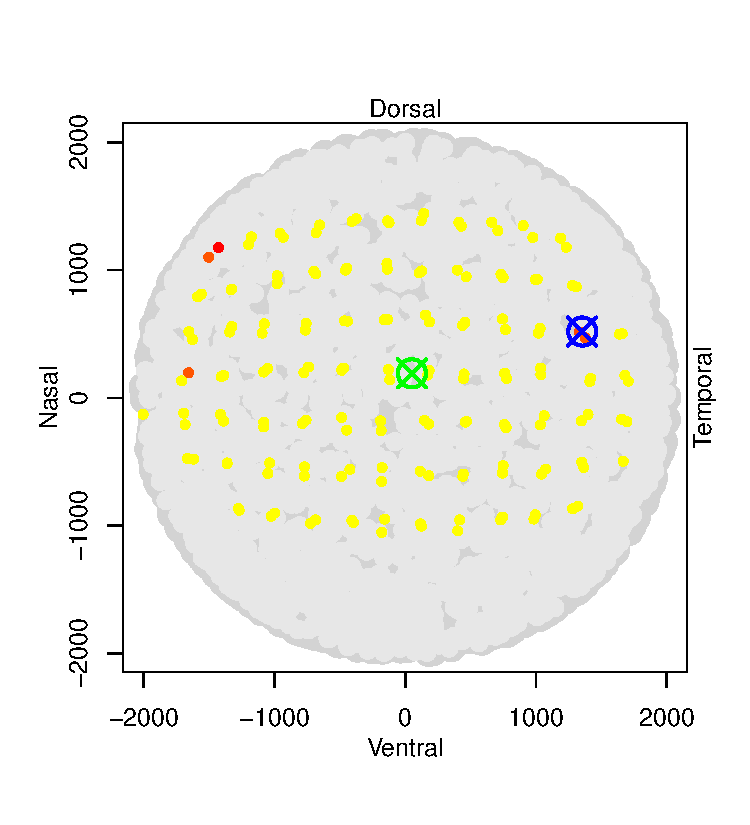
\includegraphics{/Users/kiehlt/Documents/github-projects/RSCC-Eye-Maps/data/pr-rescue/30A2L-fig.pdf}
\caption{Visualization of photoreceptor sparing in eye 30A2L, P90 RCS Rat}
\label{fig:30A2L}
\end{figure}

\end{center}
\begin{center}
\begin{figure}
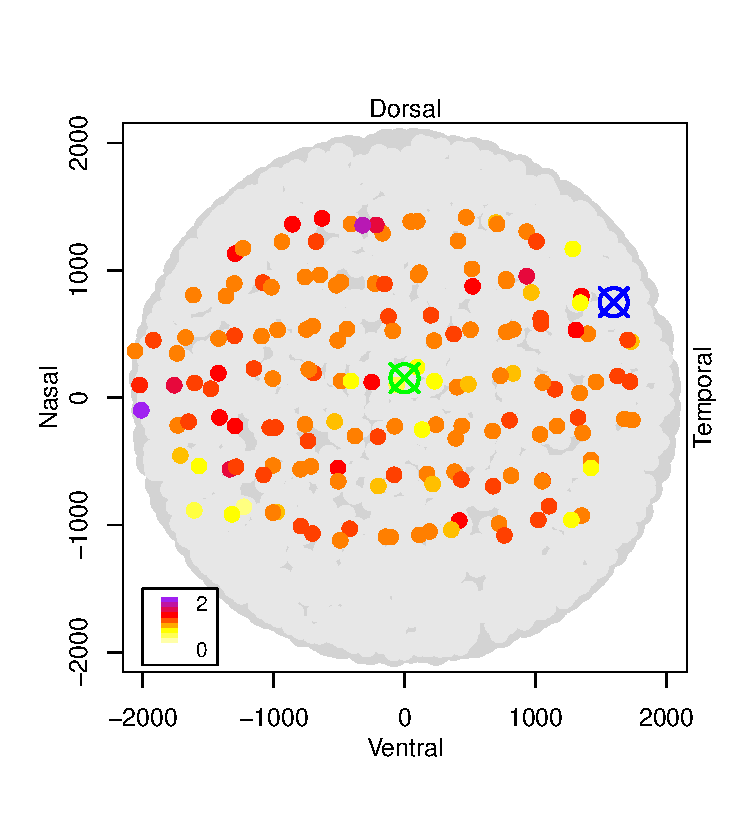
\includegraphics{/Users/kiehlt/Documents/github-projects/RSCC-Eye-Maps/data/pr-rescue/30A3L-fig.pdf}
\caption{Visualization of photoreceptor sparing in eye 30A3L, P90 RCS Rat}
\label{fig:30A3L}
\end{figure}

\end{center}
\begin{center}
\begin{figure}
\includegraphics{/Users/kiehlt/Documents/github-projects/RSCC-Eye-Maps/data/pr-rescue/30B1L-fig.pdf}
\caption{Visualization of photoreceptor sparing in eye 30B1L, P90 RCS Rat}
\label{fig:30B1L}
\end{figure}

\end{center}
\begin{center}
\begin{figure}
\includegraphics{/Users/kiehlt/Documents/github-projects/RSCC-Eye-Maps/data/pr-rescue/30D1L-fig.pdf}
\caption{Visualization of photoreceptor sparing in eye 30D1L, P90 RCS Rat}
\label{fig:30D1L}
\end{figure}

\end{center}
\begin{center}
\begin{figure}
\includegraphics{/Users/kiehlt/Documents/github-projects/RSCC-Eye-Maps/data/pr-rescue/30F1L-fig.pdf}
\caption{Visualization of photoreceptor sparing in eye 30F1L, P90 RCS Rat}
\label{fig:30F1L}
\end{figure}

\end{center}
\begin{center}
\begin{figure}
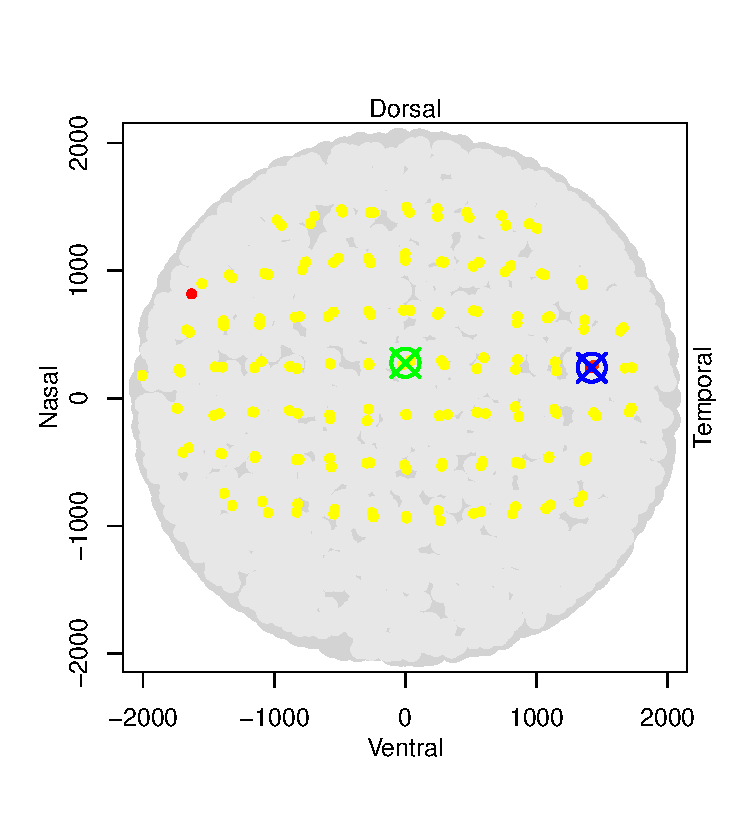
\includegraphics{/Users/kiehlt/Documents/github-projects/RSCC-Eye-Maps/data/pr-rescue/30F2L-fig.pdf}
\caption{Visualization of photoreceptor sparing in eye 30F2L, P90 RCS Rat}
\label{fig:30F2L}
\end{figure}

\end{center}
\begin{center}
\begin{figure}
\includegraphics{/Users/kiehlt/Documents/github-projects/RSCC-Eye-Maps/data/pr-rescue/30I1L-fig.pdf}
\caption{Visualization of photoreceptor sparing in eye 30I1L, P90 RCS Rat}
\label{fig:30I1L}
\end{figure}

\end{center}
\begin{center}
\begin{figure}
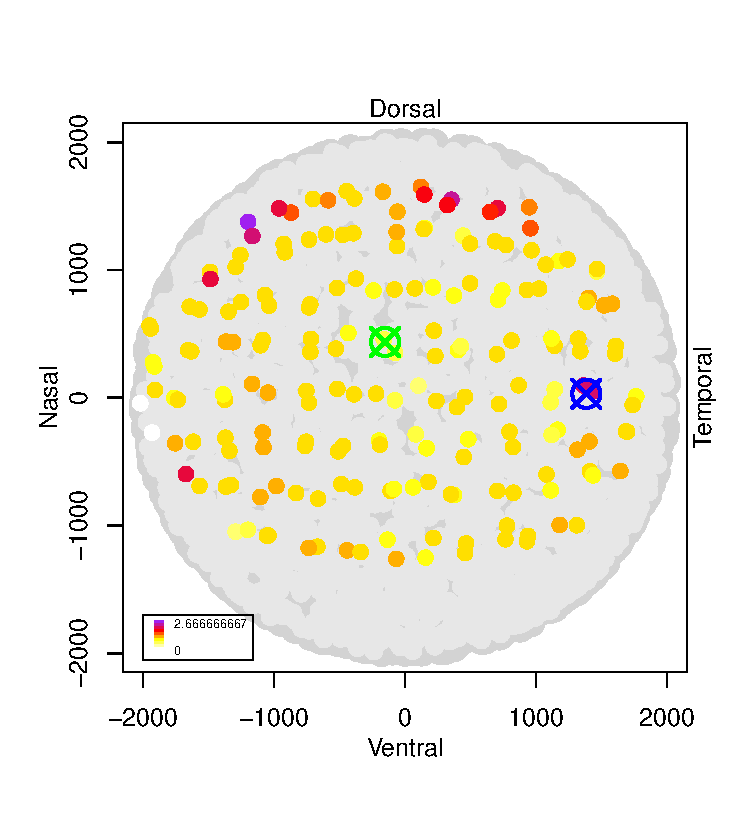
\includegraphics{/Users/kiehlt/Documents/github-projects/RSCC-Eye-Maps/data/pr-rescue/30I2L-fig.pdf}
\caption{Visualization of photoreceptor sparing in eye 30I2L, P90 RCS Rat}
\label{fig:30I2L}
\end{figure}

\end{center}
\begin{center}
\begin{figure}
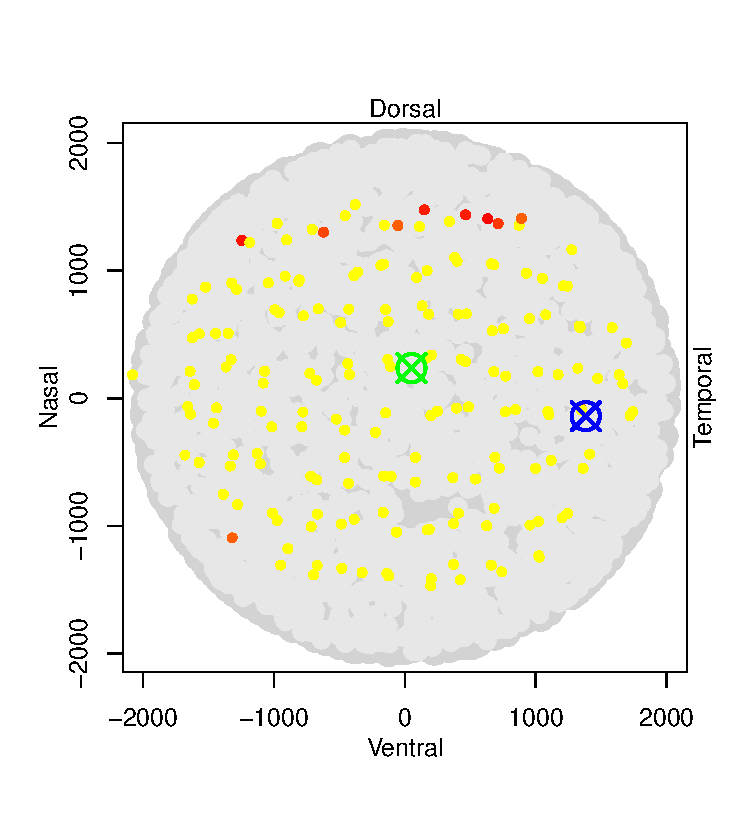
\includegraphics{/Users/kiehlt/Documents/github-projects/RSCC-Eye-Maps/data/pr-rescue/30J2L-fig.pdf}
\caption{Visualization of photoreceptor sparing in eye 30J2L, P90 RCS Rat}
\label{fig:30J2L}
\end{figure}

\end{center}
\begin{center}
\begin{figure}
\includegraphics{/Users/kiehlt/Documents/github-projects/RSCC-Eye-Maps/data/pr-rescue/30K1L-fig.pdf}
\caption{Visualization of photoreceptor sparing in eye 30K1L, P90 RCS Rat}
\label{fig:30K1L}
\end{figure}

\end{center}
\begin{center}
\begin{figure}
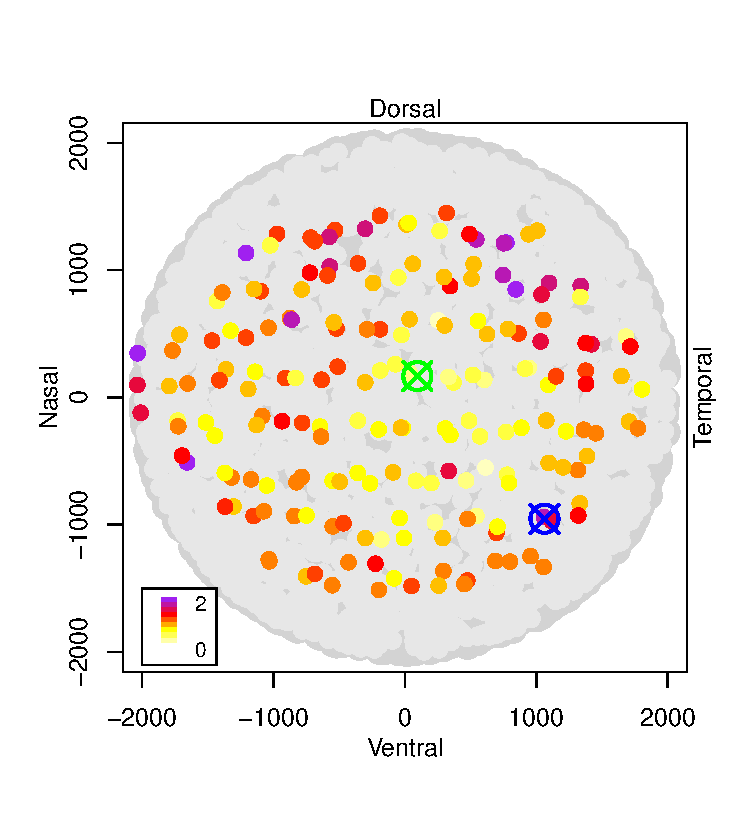
\includegraphics{/Users/kiehlt/Documents/github-projects/RSCC-Eye-Maps/data/pr-rescue/30L2L-fig.pdf}
\caption{Visualization of photoreceptor sparing in eye 30L2L, P90 RCS Rat}
\label{fig:30L2L}
\end{figure}

\end{center}
\begin{center}
\begin{figure}
\includegraphics{/Users/kiehlt/Documents/github-projects/RSCC-Eye-Maps/data/pr-rescue/30M2L-fig.pdf}
\caption{Visualization of photoreceptor sparing in eye 30M2L, P90 RCS Rat}
\label{fig:30M2L}
\end{figure}

\end{center}
\begin{center}
\begin{figure}
\includegraphics{/Users/kiehlt/Documents/github-projects/RSCC-Eye-Maps/data/pr-rescue/33A1L-fig.pdf}
\caption{Visualization of photoreceptor sparing in eye 33A1L, P150 RCS Rat}
\label{fig:33A1L}
\end{figure}

\end{center}
\begin{center}
\begin{figure}
\includegraphics{/Users/kiehlt/Documents/github-projects/RSCC-Eye-Maps/data/pr-rescue/33A2L-fig.pdf}
\caption{Visualization of photoreceptor sparing in eye 33A2L, P150 RCS Rat}
\label{fig:33A2L}
\end{figure}

\end{center}
\begin{center}
\begin{figure}
\includegraphics{/Users/kiehlt/Documents/github-projects/RSCC-Eye-Maps/data/pr-rescue/33B2L-fig.pdf}
\caption{Visualization of photoreceptor sparing in eye 33B2L, P150 RCS Rat}
\label{fig:33B2L}
\end{figure}

\end{center}
\begin{center}
\begin{figure}
\includegraphics{/Users/kiehlt/Documents/github-projects/RSCC-Eye-Maps/data/pr-rescue/33C1L-fig.pdf}
\caption{Visualization of photoreceptor sparing in eye 33C1L, P150 RCS Rat}
\label{fig:33C1L}
\end{figure}

\end{center}
\begin{center}
\begin{figure}
\includegraphics{/Users/kiehlt/Documents/github-projects/RSCC-Eye-Maps/data/pr-rescue/33D2L-fig.pdf}
\caption{Visualization of photoreceptor sparing in eye 33D2L, P150 RCS Rat}
\label{fig:33D2L}
\end{figure}

\end{center}
\begin{center}
\begin{figure}
\includegraphics{/Users/kiehlt/Documents/github-projects/RSCC-Eye-Maps/data/pr-rescue/33H3L-fig.pdf}
\caption{Visualization of photoreceptor sparing in eye 33H3L, P150 RCS Rat}
\label{fig:33H3L}
\end{figure}

\end{center}
\begin{center}
\begin{figure}
\includegraphics{/Users/kiehlt/Documents/github-projects/RSCC-Eye-Maps/data/pr-rescue/33K1L-fig.pdf}
\caption{Visualization of photoreceptor sparing in eye 33K1L, P150 RCS Rat}
\label{fig:33K1L}
\end{figure}

\end{center}
\begin{center}
\begin{figure}
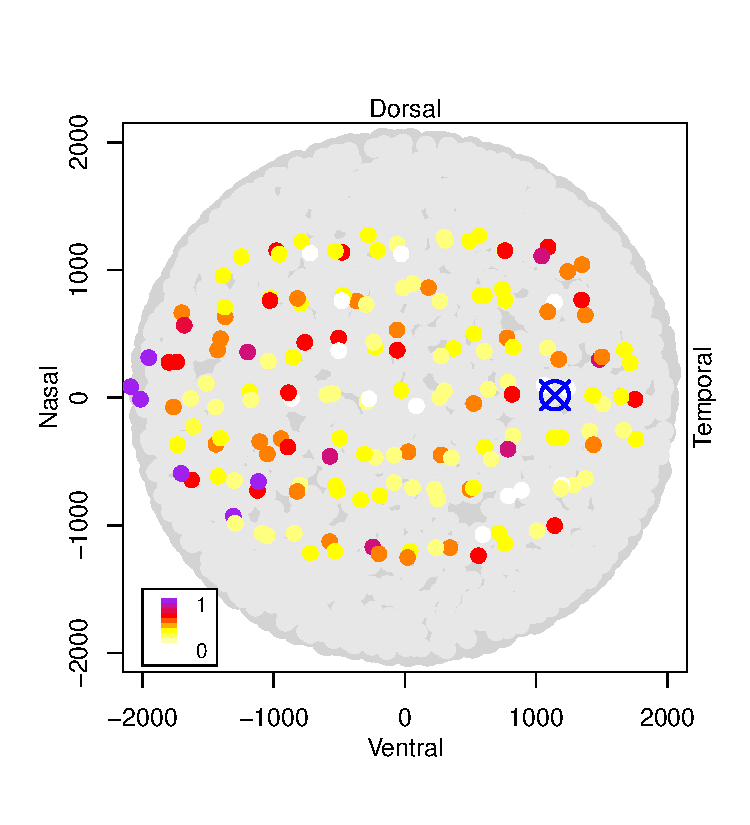
\includegraphics{/Users/kiehlt/Documents/github-projects/RSCC-Eye-Maps/data/pr-rescue/36aA3L-fig.pdf}
\caption{Visualization of photoreceptor sparing in eye 36aA3L, P180 RCS Rat}
\label{fig:36aA3L}
\end{figure}

\end{center}
\begin{center}
\begin{figure}
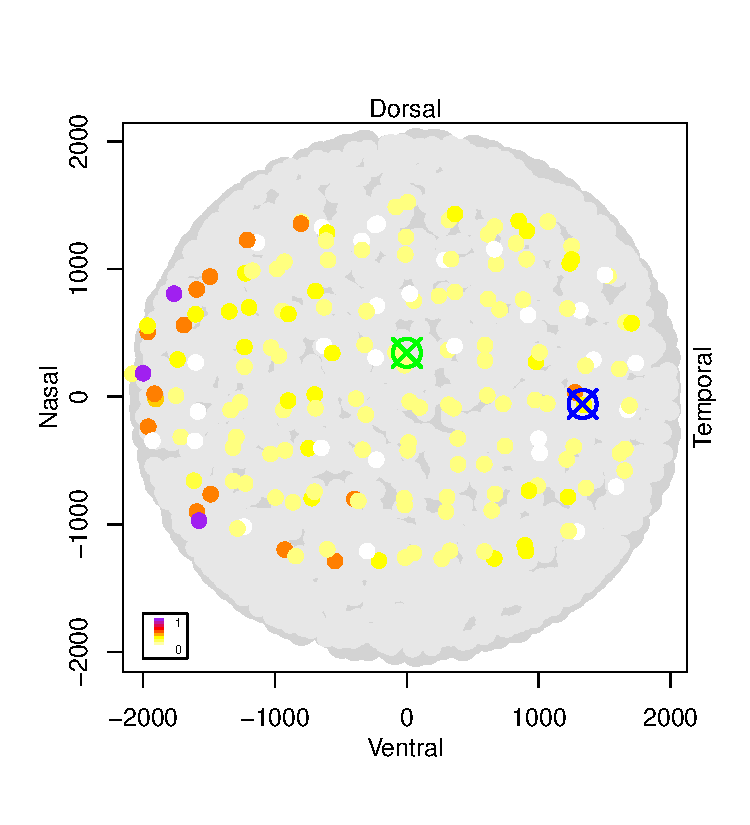
\includegraphics{/Users/kiehlt/Documents/github-projects/RSCC-Eye-Maps/data/pr-rescue/36aB3L-fig.pdf}
\caption{Visualization of photoreceptor sparing in eye 36aB3L, P180 RCS Rat}
\label{fig:36aB3L}
\end{figure}

\end{center}
\begin{center}
\begin{figure}
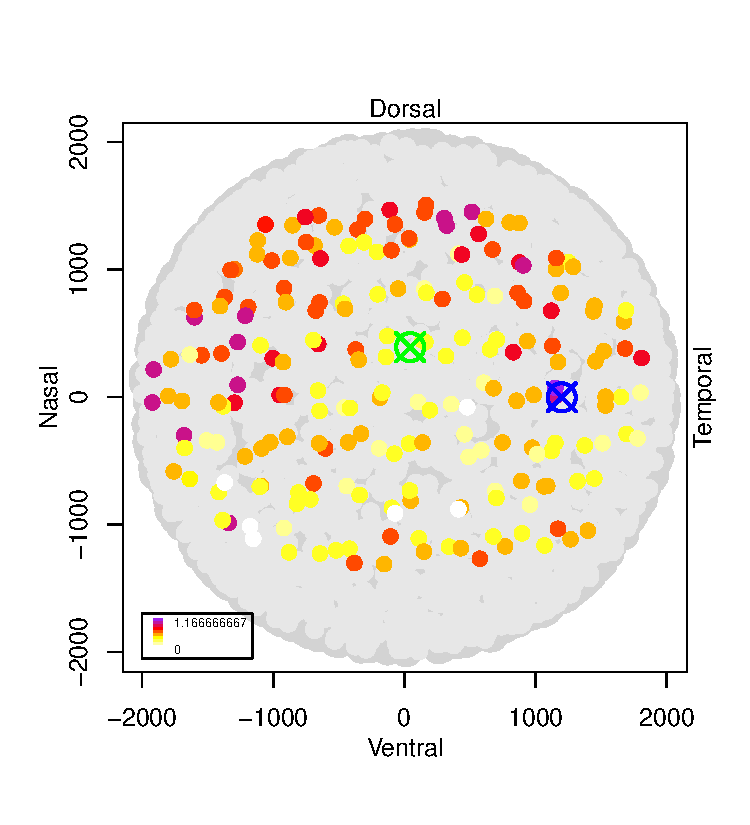
\includegraphics{/Users/kiehlt/Documents/github-projects/RSCC-Eye-Maps/data/pr-rescue/36aC3L-fig.pdf}
\caption{Visualization of photoreceptor sparing in eye 36aC3L, P180 RCS Rat}
\label{fig:36aC3L}
\end{figure}

\end{center}
\begin{center}
\begin{figure}
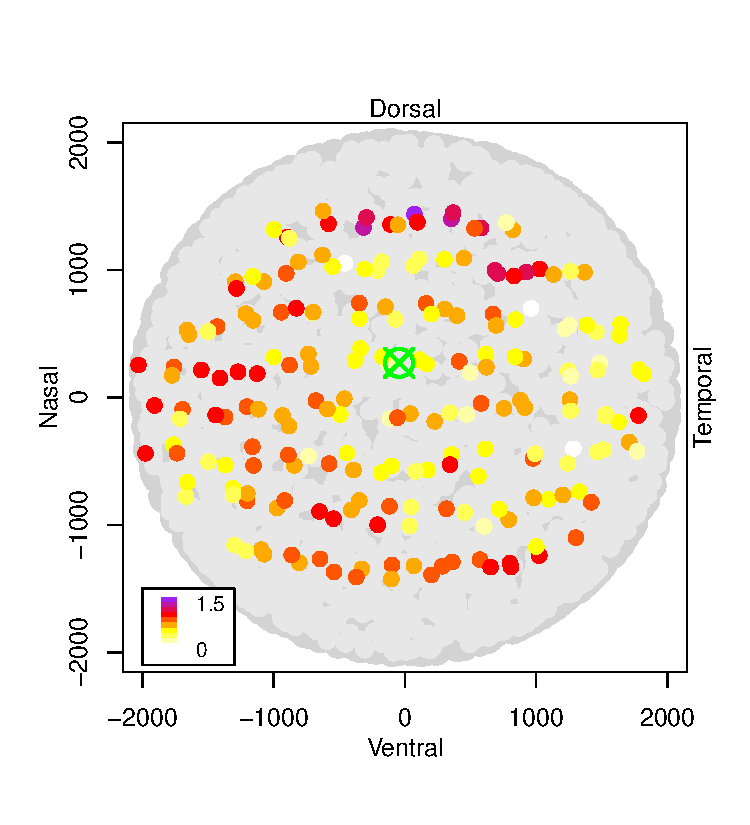
\includegraphics{/Users/kiehlt/Documents/github-projects/RSCC-Eye-Maps/data/pr-rescue/36aE2L-fig.pdf}
\caption{Visualization of photoreceptor sparing in eye 36aE2L, P180 RCS Rat}
\label{fig:36aE2L}
\end{figure}

\end{center}
\begin{center}
\begin{figure}
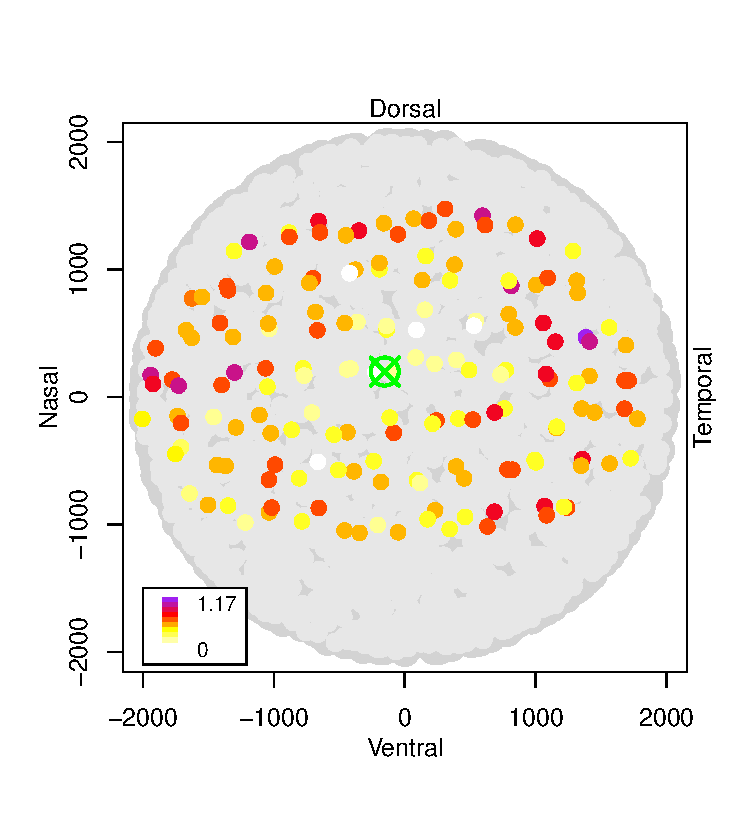
\includegraphics{/Users/kiehlt/Documents/github-projects/RSCC-Eye-Maps/data/pr-rescue/36aF2L-fig.pdf}
\caption{Visualization of photoreceptor sparing in eye 36aF2L, P180 RCS Rat}
\label{fig:36aF2L}
\end{figure}

\end{center}
\begin{center}
\begin{figure}
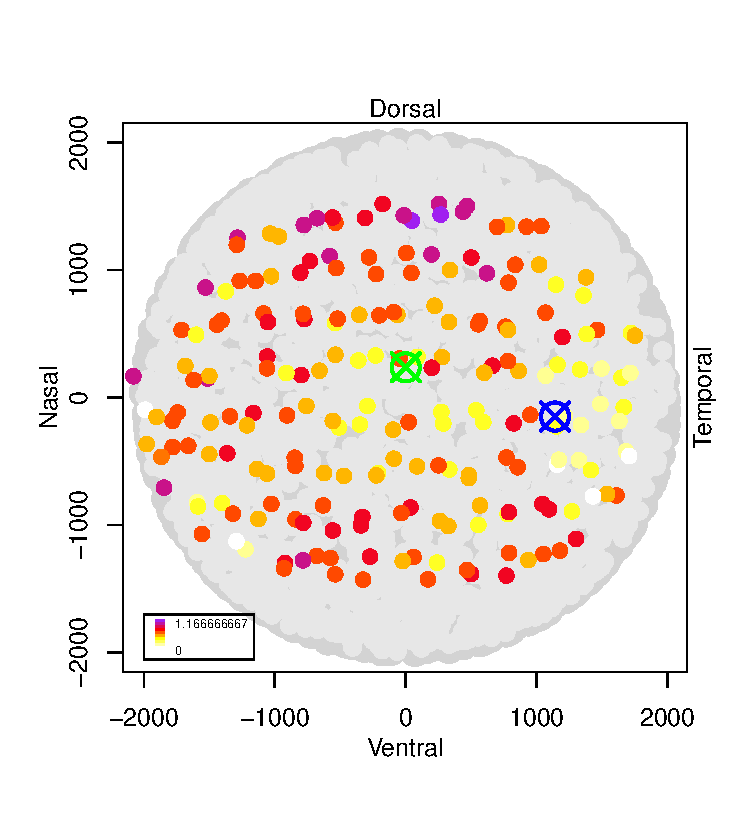
\includegraphics{/Users/kiehlt/Documents/github-projects/RSCC-Eye-Maps/data/pr-rescue/36aF3L-fig.pdf}
\caption{Visualization of photoreceptor sparing in eye 36aF3L, P180 RCS Rat}
\label{fig:36aF3L}
\end{figure}

\end{center}
\begin{center}
\begin{figure}
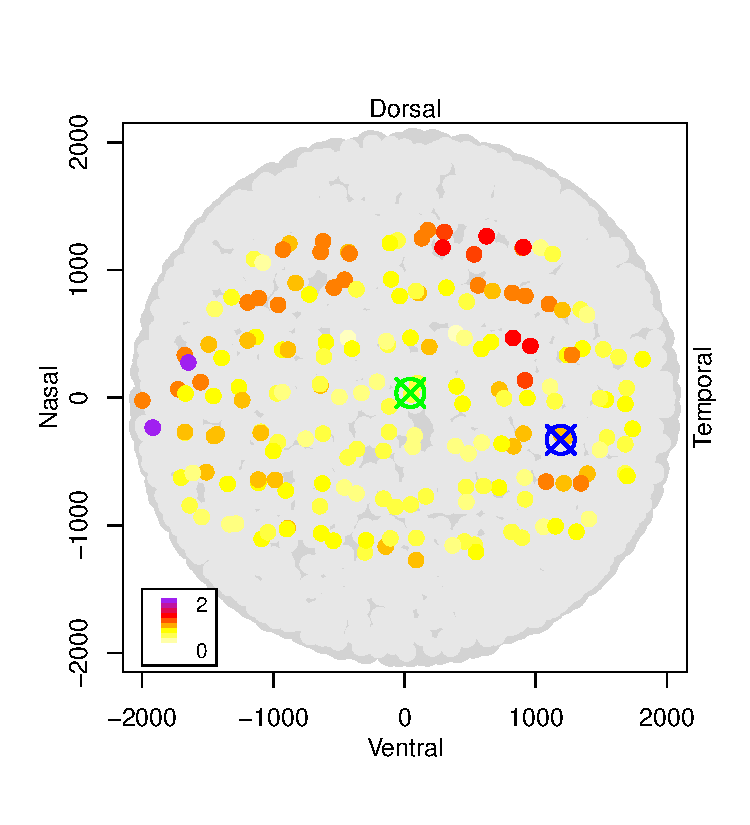
\includegraphics{/Users/kiehlt/Documents/github-projects/RSCC-Eye-Maps/data/pr-rescue/36aG1L-fig.pdf}
\caption{Visualization of photoreceptor sparing in eye 36aG1L, P180 RCS Rat}
\label{fig:36aG1L}
\end{figure}

\end{center}
\begin{center}
\begin{figure}
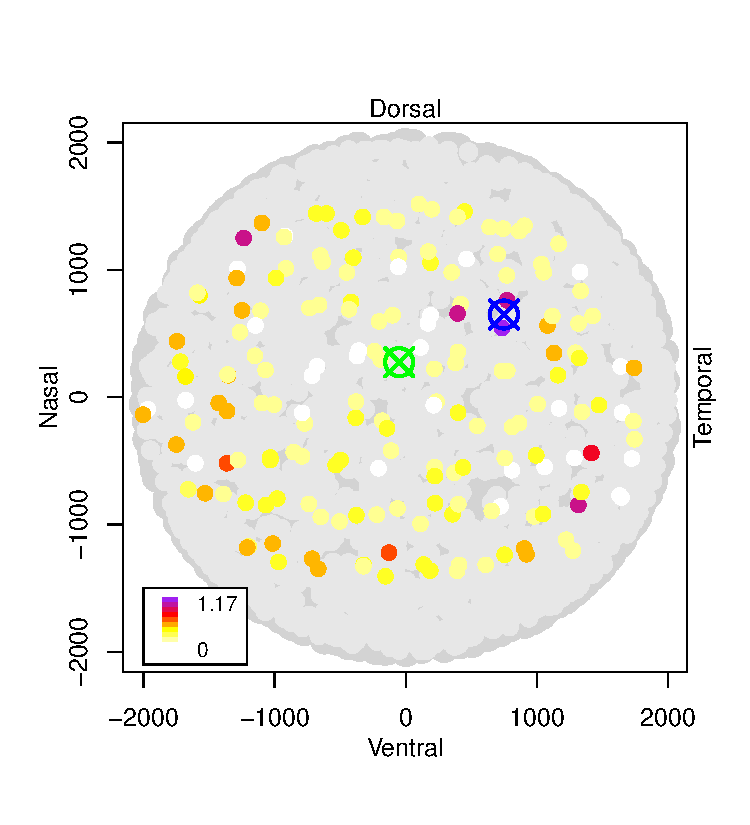
\includegraphics{/Users/kiehlt/Documents/github-projects/RSCC-Eye-Maps/data/pr-rescue/36aG3L-fig.pdf}
\caption{Visualization of photoreceptor sparing in eye 36aG3L, P180 RCS Rat}
\label{fig:36aG3L}
\end{figure}

\end{center}
\begin{center}
\begin{figure}
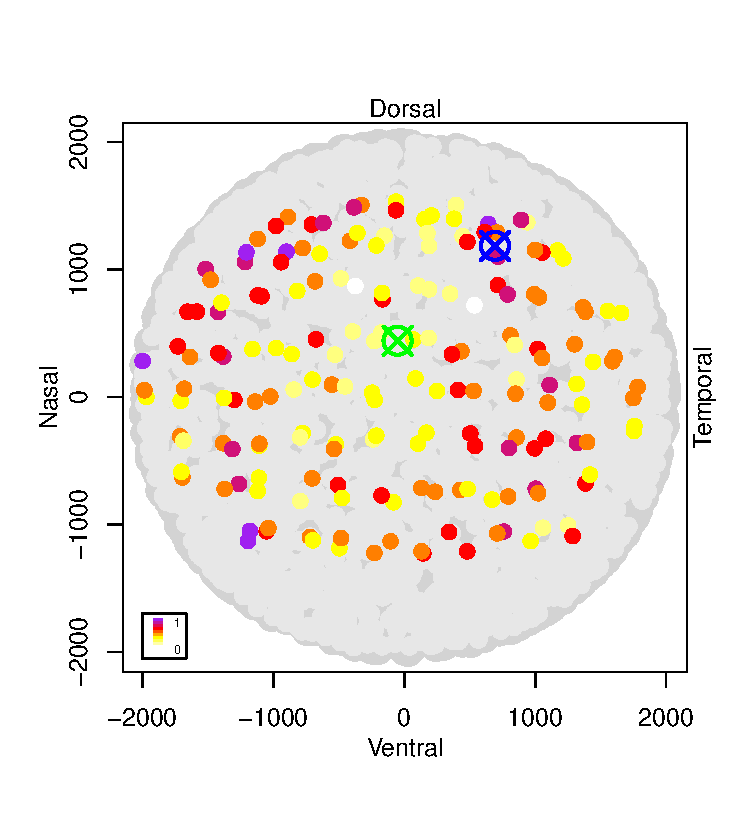
\includegraphics{/Users/kiehlt/Documents/github-projects/RSCC-Eye-Maps/data/pr-rescue/36aH1L-fig.pdf}
\caption{Visualization of photoreceptor sparing in eye 36aH1L, P180 RCS Rat}
\label{fig:36aH1L}
\end{figure}

\end{center}
\begin{center}
\begin{figure}
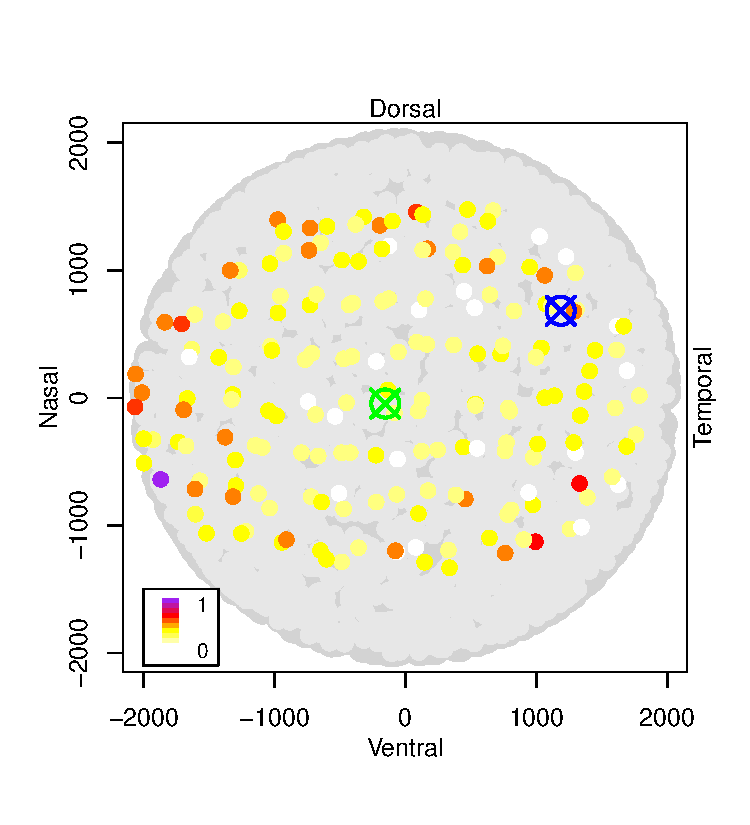
\includegraphics{/Users/kiehlt/Documents/github-projects/RSCC-Eye-Maps/data/pr-rescue/36bI2L-fig.pdf}
\caption{Visualization of photoreceptor sparing in eye 36bI2L, P180 RCS Rat}
\label{fig:36bI2L}
\end{figure}

\end{center}
\begin{center}
\begin{figure}
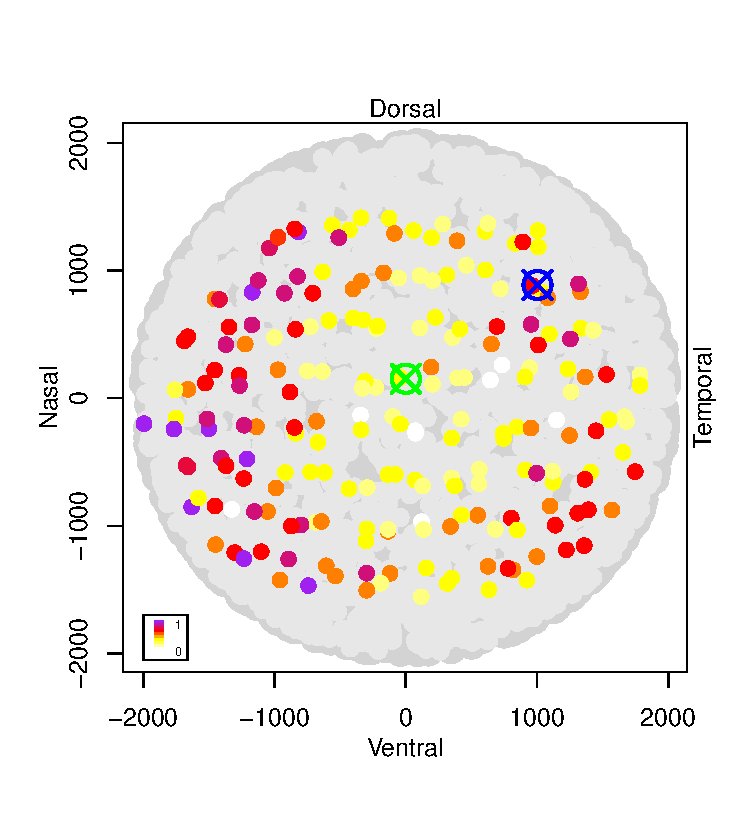
\includegraphics{/Users/kiehlt/Documents/github-projects/RSCC-Eye-Maps/data/pr-rescue/36bK2L-fig.pdf}
\caption{Visualization of photoreceptor sparing in eye 36bK2L, P180 RCS Rat}
\label{fig:36bK2L}
\end{figure}

\end{center}
\begin{center}
\begin{figure}
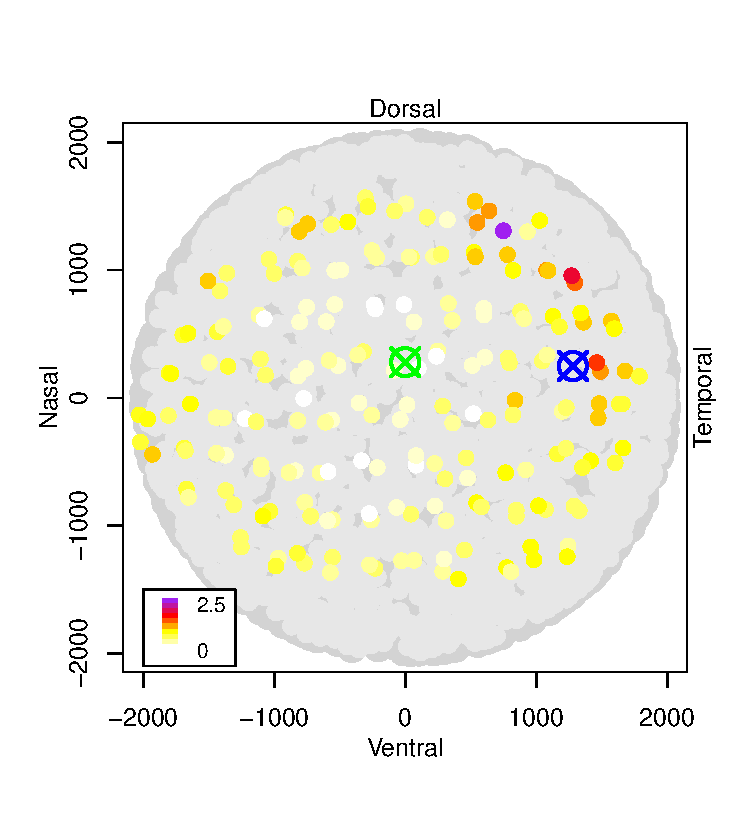
\includegraphics{/Users/kiehlt/Documents/github-projects/RSCC-Eye-Maps/data/pr-rescue/36bL2L-fig.pdf}
\caption{Visualization of photoreceptor sparing in eye 36bL2L, P180 RCS Rat}
\label{fig:36bL2L}
\end{figure}

\end{center}\newpage

\section{Experiment 26 - Validation}
Note that no 3002 records were available for experiment 26. As such,tghe injection site and optic nerve are not labeled. Only the HLA observations are rendered herein.
\subsection{HLA Figures for Validation Study - Experiment 26}
HLA observations were collected for the following eyes.
\begin{table}[]
\centering
\begin{tabular}{l}
\textbf{Exp 26 (RNU Rats Terminated at 9 Months) } \\
26DB1L -  Injected with 20\% RPE and 80\% EMT cells \\
26DC1L - Injected with 20\% RPE and 80\% EMT cells \\
26F2L - Injected with 100\% RPE and 0\% EMT cells \\
26DG1L -  Injected with 0\% RPE and 100\% EMT cells  \\
26DG2L -  Injected with 0\% RPE and 100\% EMT cells\\
\end{tabular}
\caption{Experiments counted for HLA Mapping}
\label{tab:exp26}
\end{table}

All of the plots here use follow the same conventions as the above HLA plots. Total number of sections comprising each eye can be found in the above table \ref{tab:sectioncounttable}.

\begin{center}
\begin{figure}
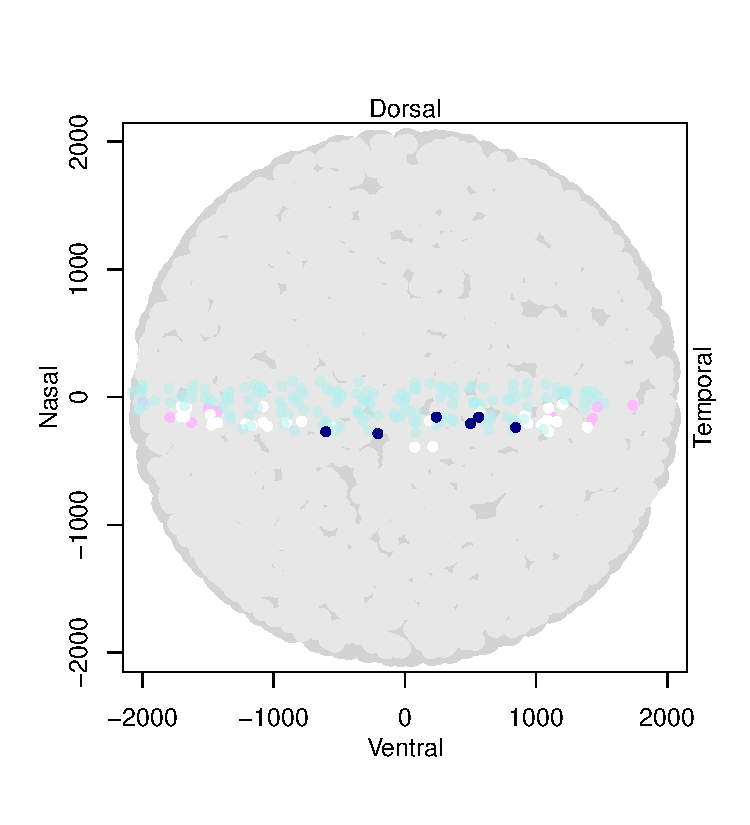
\includegraphics{/Users/kiehlt/Documents/github-projects/RSCC-Eye-Maps/data/hla-mapping/26DB1L-fig.pdf}
\caption{Visualization of HLA mapping in eye 26DB1L, RNU rat  injected with 20\% RPE and 80\% EMT cells. Animal terminated at 9 months.}
\label{fig:26DB1L}
\end{figure}

\end{center}
\begin{center}
\begin{figure}
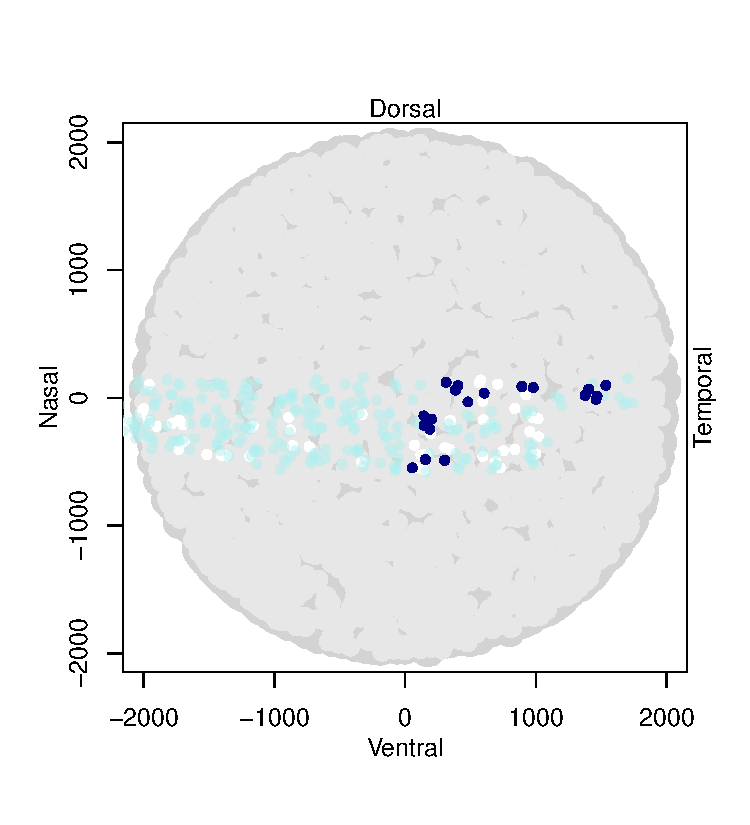
\includegraphics{/Users/kiehlt/Documents/github-projects/RSCC-Eye-Maps/data/hla-mapping/26DC1L-fig.pdf}
\caption{Visualization of HLA mapping in eye 26DC1L, RNU rat injected with 20\% RPE and 80\% EMT cells. Animal terminated at 9 months.}
\label{fig:26DC1L}
\end{figure}

\end{center}
\begin{center}
\begin{figure}
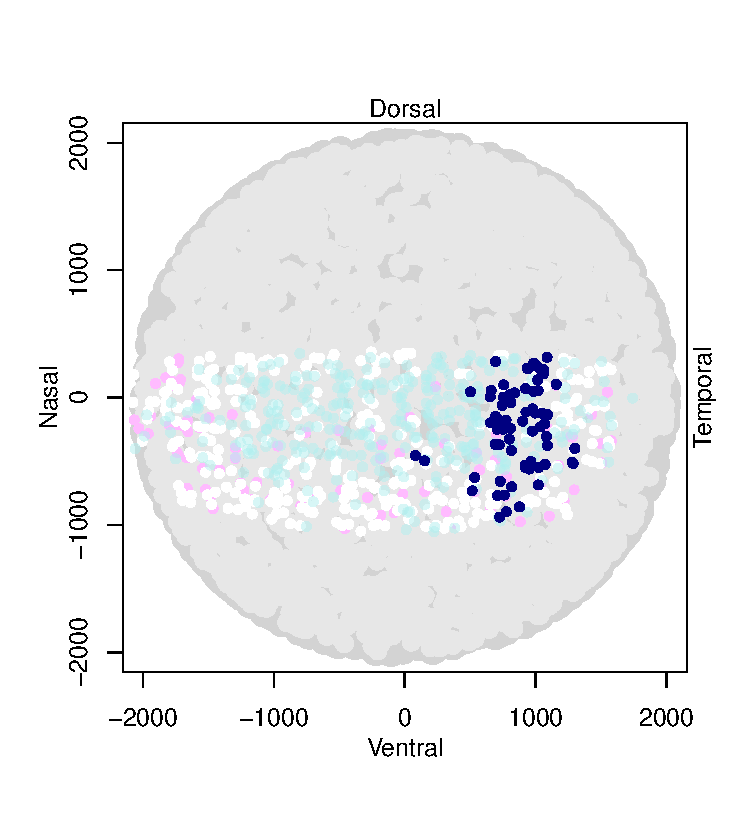
\includegraphics{/Users/kiehlt/Documents/github-projects/RSCC-Eye-Maps/data/hla-mapping/26DF2L-fig.pdf}
\caption{Visualization of HLA mapping in eye 26DF2L, RNU rat injected with 100\% RPE and 0\% EMT cells. Animal terminated at 9 months.}
\label{fig:26DF2L}
\end{figure}

\end{center}
\begin{center}
\begin{figure}
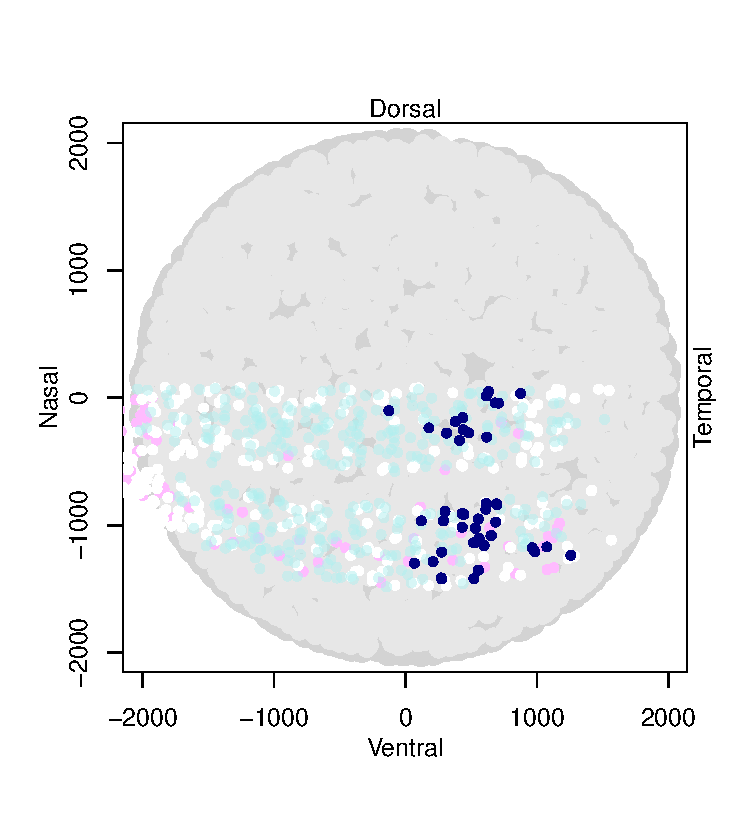
\includegraphics{/Users/kiehlt/Documents/github-projects/RSCC-Eye-Maps/data/hla-mapping/26DG1L-fig.pdf}
\caption{Visualization of HLA mapping in eye 26DG1L, RNU rat injected with 0\% RPE and 100\% EMT cells. Animal terminated at 9 months.}
\label{fig:26DG1L}
\end{figure}

\end{center}
\begin{center}
\begin{figure}
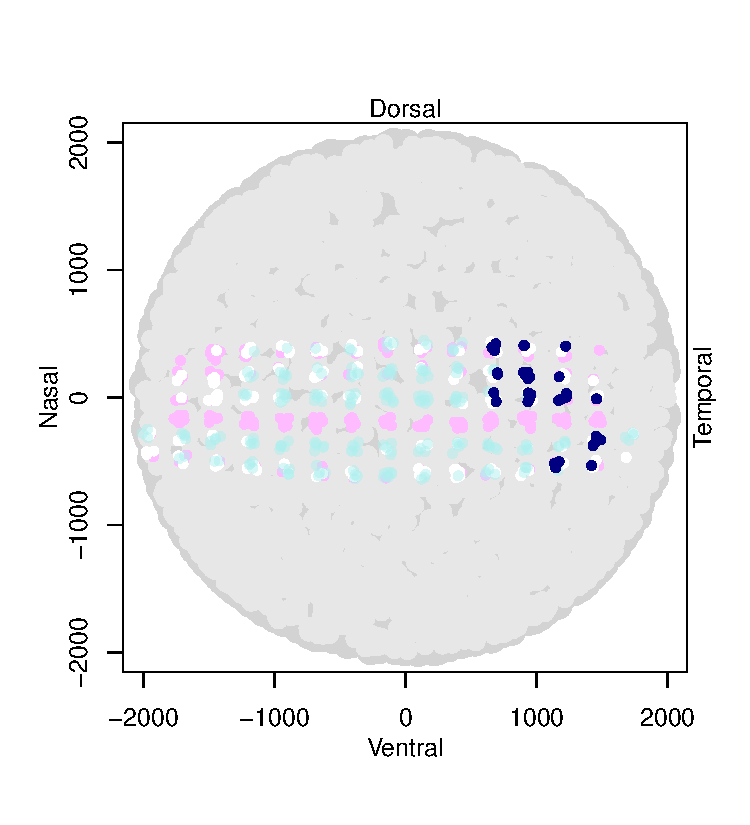
\includegraphics{/Users/kiehlt/Documents/github-projects/RSCC-Eye-Maps/data/hla-mapping/26DG2L-fig.pdf}
\caption{Visualization of HLA mapping in eye 26DG2L, RNU rat injected with 0\% RPE and 100\% EMT cells. Animal terminated at 9 months.}
\label{fig:26DG2L}
\end{figure}

\end{center}
\end{document}
